\section{Data acquisition}
\writer{Matthew Wing, Taikan Suehara}{2}

The ILD data acquisition takes advantage of the relatively low rate of relevant physics $e^+e^-$ interactions (O(0.1 hadronic evt)/BC) and of the long idle periods between bunch trains (chapter 3) to provide a triggerless readout of the detector. The subdetector data of all BCs of a given bunch train are collected before the next bunch train and processed offline as a single data set for identification, bunch tagging and reconstruction of the individual interactions. 


\subsection{DAQ architecture}

The overall organisation of the DAQ system is summarized in Figure~\ref{fig:integration:DAQ_architecture}. 

\begin{figure}[t!]
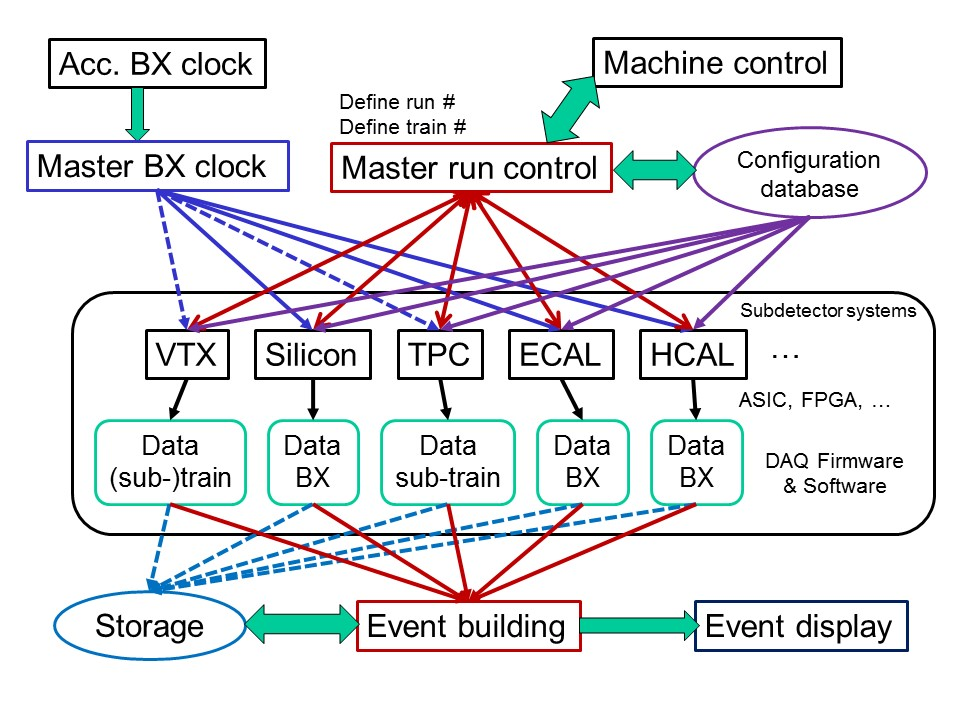
\includegraphics[width=1.0\hsize]{Integration/fig/DAQ_architecture.jpg}
\caption{\label{fig:integration:DAQ_architecture}Global architecture of the ILD data acquisition system.}
\end{figure}

The processing of subdetector data is first performed locally with a high parallelism within FPGA and ASIC boards which each typically treat O(100) subdetector channels. The individual data are zero-suppressed, amplified, time stamped and digitized, depending on the subdetector, and stored in local pipelines dimensioned adequately for a full bunch train. The "event building" is performed between bunch trains by gathering all subdetector data of a given bunch train into a single bunch train data set. The bunch train data sets are stored locally on the IP Campus (section 6.2.1) and transferred to an offline computing farm which may be located on the main campus. In the farm each bunch train data set is processed individually by one processor in order to identify individual events, tag their bunch crossings and perform calibration and reconstruction. This scheme caters for the different time resolutions of the subdetectors, which range from individual bunch tagging as done e.g. in the calorimeters, to a full train integration time as in the TPC.

One critical component of the system is the clock distribution to the subdetector front-ends: this has to be done on the overall ILD detector with a precision better than 10 ps to enable time-of-flight measurements. On the other hand the overall data flow requirements are moderate. They have not changed significantly compared to the estimates reported in [DBD], and correspond to a raw data rate of O(100MB)/train for a storage data size of O(10PB)/year. The data flow is dominated by high granularity detectors exposed to high beam background close to the beampipe (Vertex and Beamcal). If needed it could be further reduced by local partial event processing ahead of the event building.

\subsection{DAQ R\&D}

The front-end processing has benefited from the development of subdetector technological prototypes including final readout front-end components as reported in section 5.2. ASIC and FPGA boards with the required ILD specifications are now available for most subdetectors.

A number of common DAQ aspects relevant for the final ILD central DAQ have been developed \cite{ild:bib:AIDADAQ} within the AIDA-2020 programme. They include both hardware and software components which have been used for different detectors or combinations of detectors in beam tests involving not only ILD prototypes but also detectors developed for the HL-LHC. 

The core hardware component of the central DAQ system, the Trigger Logic Unit (TLU), provides a common interface for synchronisation and control of subdetectors. A new TLU has been developed to distribute signals to multiple detectors in beam tests. The AIDA-2020 TLU (Figure~\ref{fig:integration:DAQ_TLU}) has been extended over the previous version to be able to synchronise detectors with differing trigger and readout schemes, such as the CALICE calorimeters, pixel detectors and tracking devices, as well as being able to operate at a higher particle flux. Therefore, data from different detectors corresponding to the same particle in a test beam can be combined. The TLU is used extensively in test-beam facilities at CERN and DESY and will continue to do so thereby serving the needs of many detectors also beyond ILC R\&D. 

\begin{figure}[t!]
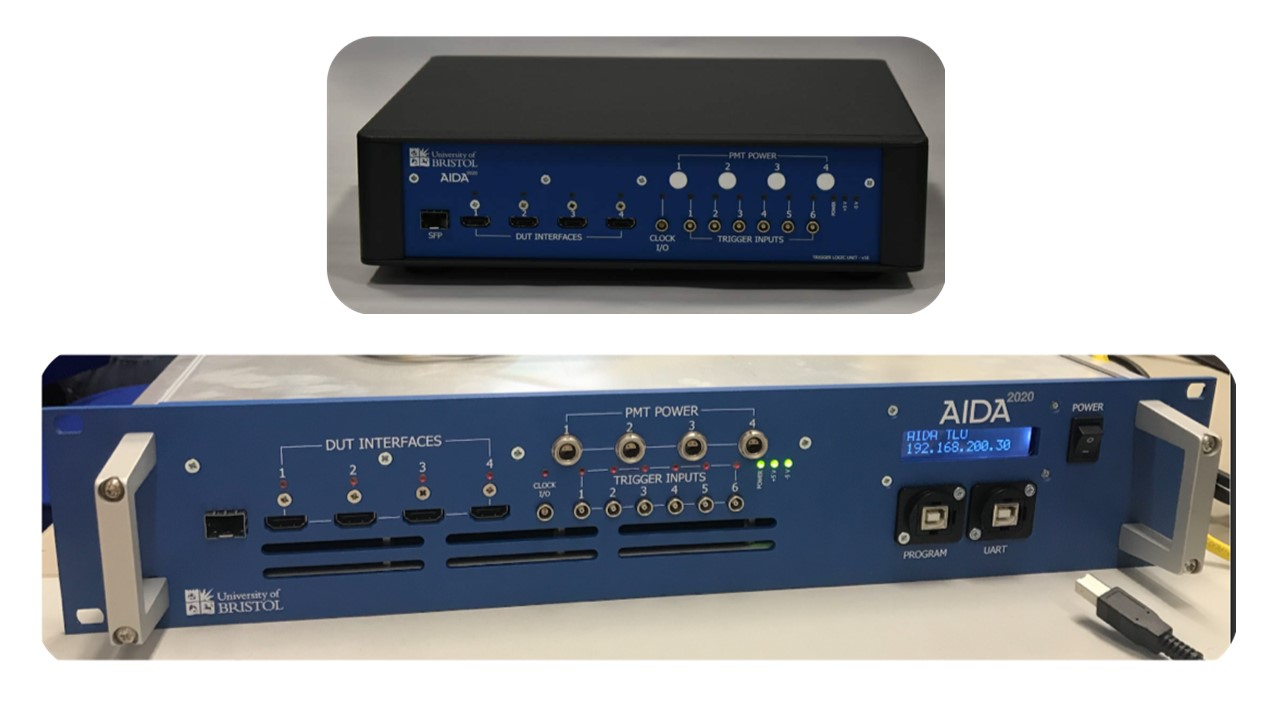
\includegraphics[width=1.0\hsize]{Integration/fig/DAQ_TLU.jpg}
\caption{\label{fig:integration:DAQ_TLU}The AIDA-2020 newly developed Trigger Logic Unit. Top: table top enclosure. Bottom: 19-inch rack-mounted enclosure. The two enclosures have identical inner components and provide the same functionalities.}
\end{figure}

Within AIDA-2020 DAQ software packages have also been developed for both data collection and monitoring. The EUDAQ2 software is an extension of the EUDAQ software developed for the EUDET pixel beam telescope. It supports detectors with different trigger schemes and different readout speeds, enabling combined beam tests of very different detectors to be performed. The software has been tested and used in several beam tests so far, notably for the AHCAL (also in conjunction with the CMS HGCAL), and for tracker modules of the ATLAS upgrade.  The TLU is also fully integrated into the EUDAQ2 framework. The monitoring software, DQM4HEP, originally developed for the SDHCAL, has been used for data quality monitoring and slow control monitoring. This software is a generic development which has extendibility built in and so can be used to monitor data from any detector in any format. It has already been successfully used by the AHCAL+beam telescope and SDHCAL+SiW-ECAL combined beam tests. 

These DAQ developments have allowed multiple detectors to be more easily integrated, sparing time for understanding technical aspects of the detector technologies and the physics performances.  Further detector developments will also benefit from this. The work also informs our understanding of integration and DAQ issues for the final ILD.

\vspace{2cm}
